\chapter{La diferenciación celular: la célula muscular esquelética}\label{ch:b2:cell-differentiation}

Una fibra del músculo del muslo es una sola célula de treinta centímetros
de largo, con cientos de núcleos, llena de un extremo a otro de varillas
contráctiles tan regulares que al microscopio se ve estriada. Empezó
siendo un grupo de células de aspecto corriente que salieron reptando de
un somito, se multiplicaron, dejaron de dividirse, se alinearon, se
fusionaron y activaron varios cientos de genes que nunca habían usado. Todas
las células del cuerpo tienen el mismo genoma; una \omterm{def:b2:cell-differentiation:myogenesis}{fibra muscular} es lo
que hace ese genoma cuando se activa un \omterm{prop:b2:cell-differentiation:transcriptional}{factor de transcripción} concreto.
Este capítulo toma la célula muscular esquelética como ejemplo resuelto de
\emph{\omterm{def:b2:cell-differentiation:differentiation}{diferenciación}} --- cómo adquiere y conserva una célula una identidad
especializada ---, y la célula muscular es un buen ejemplo porque se conoce
su interruptor maestro, sus etapas pueden observarse en una placa y la
célula terminada es una máquina cuyas piezas están a la vista.

\section{Qué es la diferenciación}

\begin{definition}[Diferenciación, determinación, potencia]\label{def:b2:cell-differentiation:differentiation}
\index{diferenciación}\index{determinación}\index{célula madre}\index{potencia}
Una célula está \emph{diferenciada} cuando expresa el patrón estable de
genes --- y, por tanto, las proteínas, la forma y la función --- de un tipo
celular. Está \emph{determinada} (o comprometida) cuando su destino está
fijado aunque su diferenciación aún no haya empezado: un \omterm{def:b2:cell-differentiation:myogenesis}{mioblasto} parece
un fibroblasto, pero solo formará músculo. La \emph{potencia} es el
abanico de tipos que una célula todavía puede dar: \emph{totipotente} (el
cigoto y los primeros blastómeros, que lo forman todo, \omterm{def:b2:mammal-reproduction:placenta}{placenta}
incluida), \emph{pluripotente} (la \omterm{def:b2:mammal-reproduction:implantation}{masa celular interna}, que forma todos
los tejidos del cuerpo), \emph{multipotente} (una célula madre de la
sangre o del músculo, que forma los tipos de un tejido),
\emph{unipotente}. Una \emph{célula madre} es una célula que se divide
dando una hija igual a ella y otra que pasa a diferenciarse, lo que
mantiene la reserva mientras abastece al tejido. La diferenciación no es,
en la mayoría de los casos, una pérdida de genes sino una elección entre
ellos: el genoma de un núcleo muscular está completo.
\end{definition}
\begin{proof}[Evidencia]
Gurdon (1962) trasplantó el núcleo de una célula intestinal diferenciada
de un renacuajo a un huevo de rana cuyo propio núcleo había sido
destruido; una fracción de los huevos se desarrolló en ranas normales y
fértiles. El núcleo diferenciado no había perdido ninguno de los genes
necesarios para formar un animal completo; el citoplasma del huevo lo había
reiniciado. La misma operación con un núcleo de célula mamaria en un
óvulo de oveja dio a Dolly (1996), y la reprogramación de un fibroblasto
de la piel en una \omterm{def:b2:cell-differentiation:differentiation}{célula madre} pluripotente mediante cuatro \omterm{prop:b2:cell-differentiation:transcriptional}{factores de
transcripción} (Yamanaka, 2006) mostró que el reinicio puede lograrse con
un puñado de proteínas.
\end{proof}

\begin{proposition}[La diferenciación es transcripcional]\label{prop:b2:cell-differentiation:transcriptional}
\index{factor de transcripción}\index{regulador maestro}
La diferencia entre dos tipos celulares reside en qué genes se
transcriben. Unos pocos \emph{\omterm{prop:b2:cell-differentiation:transcriptional}{factores de transcripción}}, expresados en
respuesta a las señales inductoras del
\cref{ch:b2:vertebrate-development}, se unen a las regiones reguladoras de
cientos de genes diana y los activan, mientras se desactivan los genes de
otros destinos; y como un factor de este tipo suele activar su propio gen,
el estado, una vez alcanzado, se mantiene por sí mismo. En algunos tejidos
un solo factor es un \emph{\omterm{prop:b2:cell-differentiation:transcriptional}{regulador maestro}} suficiente para imponer el
destino a una célula de otro tipo: \omterm{def:b2:cell-differentiation:myogenesis}{MyoD} para el músculo esquelético, Pax6
para el ojo, Sox9 para el cartílago. El estado se estabiliza además
mediante cambios de la cromatina --- metilación del ADN, modificación de
las histonas --- que mantienen silenciados los genes silenciados a lo largo
de las divisiones (la \emph{epigenética} del volumen del tercer año). Una
célula diferenciada recuerda, por tanto, lo que es sin ningún cambio en la
secuencia de su ADN, y esa memoria está escrita en el patrón de factores y
de cromatina, no en los genes.
\end{proposition}

\section{La formación de una fibra muscular}

\begin{definition}[Miogénesis]\label{def:b2:cell-differentiation:myogenesis}
\index{mioblasto}\index{miotubo}\index{fibra muscular}\index{MyoD}
En el embrión, unas señales procedentes del \omterm{prop:b2:vertebrate-development:neurulation}{tubo neural}, la notocorda y el
ectodermo superficial inducen a las células del dermomiotomo del somito a
expresar los factores miogénicos \emph{MyoD} y \emph{Myf5}: ahora son
\emph{mioblastos}, determinados pero todavía en división y de aspecto
anodino. Los mioblastos migran --- a los \omterm{def:b2:limb-organogenesis:bud}{esbozos de las extremidades}, por
ejemplo --- y se multiplican mientras haya factores de crecimiento (FGF).
Cuando los factores se agotan, salen del ciclo celular, expresan un
segundo factor, la \emph{miogenina}, se alinean extremo con extremo y se
\emph{fusionan}: sus membranas se funden en un único \emph{miotubo} largo
con muchos núcleos en fila. El miotubo activa los genes musculares ---
actina, miosina, troponina, tropomiosina, creatina quinasa, el receptor de
acetilcolina ---, ensambla el aparato contráctil y madura en una
\emph{fibra muscular} cuyos núcleos se sitúan en la periferia. Una fibra
nunca vuelve a dividirse; unos pocos mioblastos permanecen a su lado, en
reposo, como \emph{células satélite}, las \omterm{def:b2:cell-differentiation:differentiation}{células madre} que reparan y hacen
crecer el músculo durante toda la vida.
\end{definition}

\begin{omfigure}
\begin{tikzpicture}[every node/.style={font=\scriptsize}, >=stealth]
  % somite
  \draw[thick, fill=omProp!25] (0,0) ellipse (0.6 and 0.5); \node[below, align=center] at (0,-0.6) {somito\\(dermomiotomo)};
  \draw[->, thick] (0.7,0) -- (1.6,0) node[midway, above=0.35cm, align=center] {inducción\\Wnt, Shh};
  % myoblasts dividing
  \foreach \p in {(2.2,0.3),(2.7,-0.3),(3.2,0.3),(3.7,-0.3)} \draw[thick, fill=omDef!25] \p ellipse (0.28 and 0.18);
  \node[below, align=center] at (3.0,-0.6) {mioblastos: MyoD, Myf5\\se dividen mientras hay FGF};
  \draw[->, thick] (4.1,0) -- (5.0,0) node[midway, above=0.45cm, align=center] {retirada del FGF:\\miogenina,\\salida del ciclo};
  % aligned, fusing
  \foreach \x in {5.35,5.95,6.55,7.15} \draw[thick, fill=omDef!25] (\x,0) ellipse (0.3 and 0.16);
  \node[below, align=center] at (6.25,-0.6) {alineamiento y fusión};
  \draw[->, thick] (7.6,0) -- (8.5,0);
  % myotube
  \draw[thick, fill=omDef!15, rounded corners=6pt] (8.7,-0.3) rectangle (12.6,0.3);
  \foreach \x in {9.2,10.0,10.8,11.6,12.3} \fill[omDef!80!black] (\x,0) ellipse (0.13 and 0.08);
  \node[below, align=center] at (10.65,-0.6) {miotubo: muchos núcleos,\\genes musculares activos, miofibrillas ensambladas};
\end{tikzpicture}

{\small Miogénesis: las células inducidas del somito se convierten en
\omterm{def:b2:cell-differentiation:myogenesis}{mioblastos} en división; cuando se retiran los factores de crecimiento,
dejan de dividirse, se alinean y se fusionan en un \omterm{def:b2:cell-differentiation:myogenesis}{miotubo} multinucleado
que activa los genes musculares.}
\end{omfigure}

\begin{omfigure}
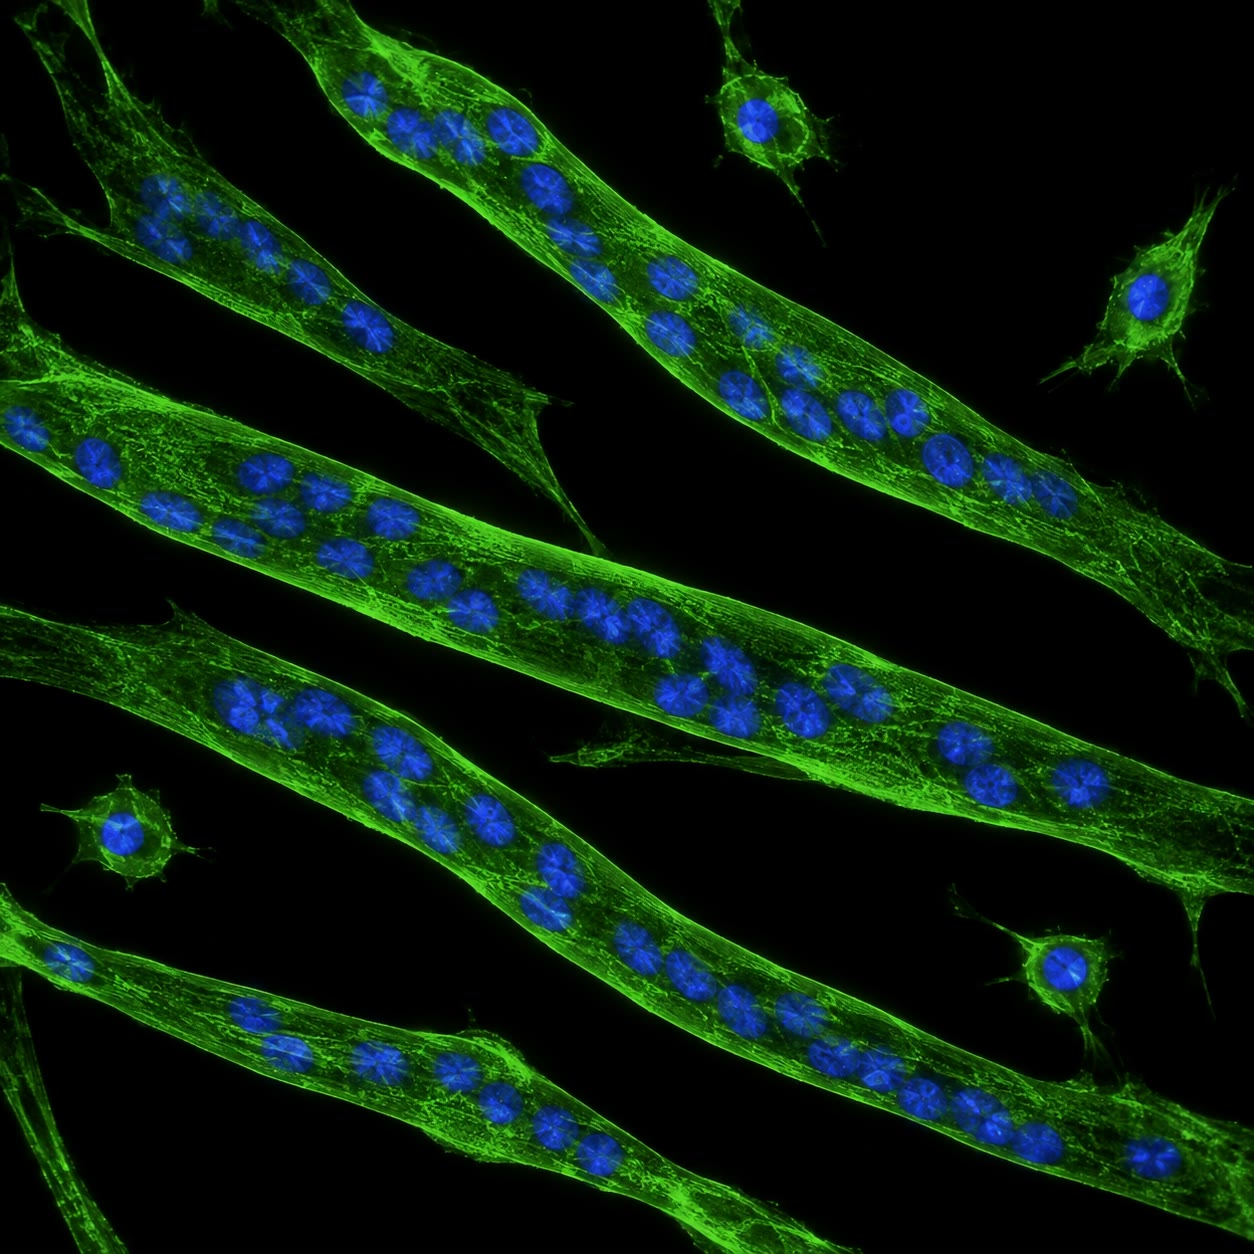
\includegraphics[width=0.44\linewidth]{images/book4/ai/b4-12-myotubes.jpg}\hspace{0.04\linewidth}
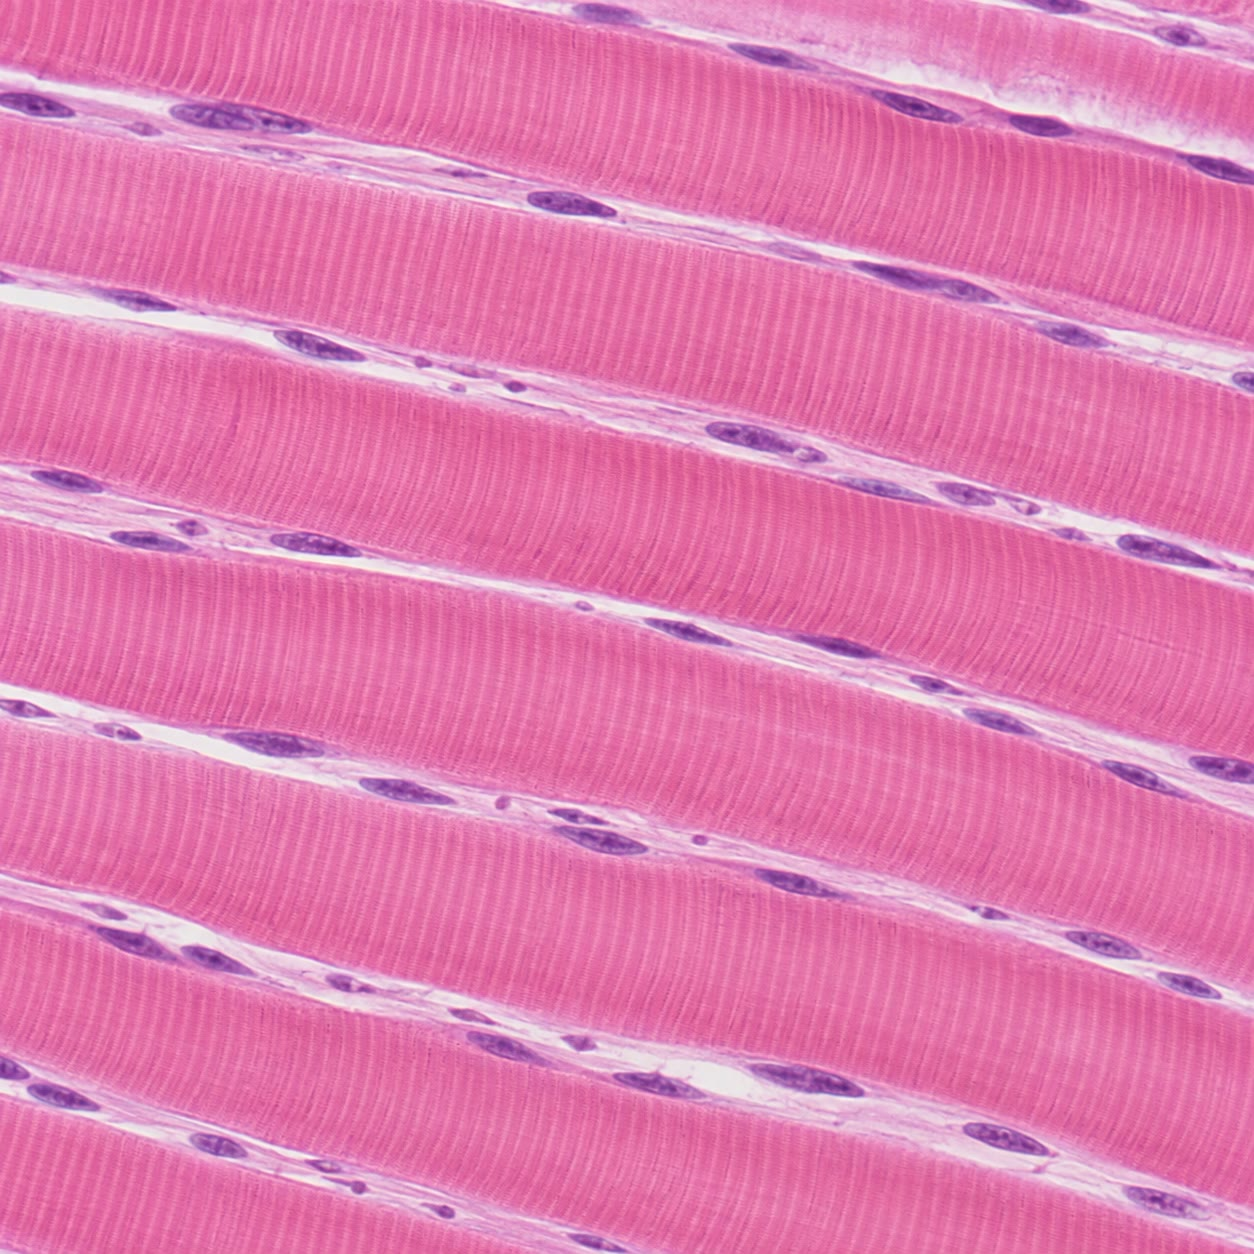
\includegraphics[width=0.44\linewidth]{images/book4/ai/b4-12-muscle-fibres.jpg}

{\small Izquierda: \omterm{def:b2:cell-differentiation:myogenesis}{miotubos} en cultivo, cada uno una célula fusionada con
una fila de núcleos, junto a \omterm{def:b2:cell-differentiation:myogenesis}{mioblastos} aislados que aún no se han
fusionado. Derecha: fibras maduras en vista longitudinal, con sus
estriaciones transversales, que son los \omterm{def:b2:cell-differentiation:fibre}{sarcómeros} repetidos, y sus
núcleos desplazados hacia el borde.}
\end{omfigure}

\begin{proposition}[MyoD: un interruptor maestro]\label{prop:b2:cell-differentiation:myod}
\index{regulador maestro!MyoD}
\omterm{def:b2:cell-differentiation:myogenesis}{MyoD} es un \omterm{prop:b2:cell-differentiation:transcriptional}{factor de transcripción} de la familia hélice-bucle-hélice. Se
une, como dímero con una proteína compañera ubicua, a una secuencia de
seis bases (la caja E, CANNTG) de las regiones reguladoras de los genes
musculares, recluta enzimas que abren la cromatina y activa los genes
--- entre ellos los de la miogenina y del propio \omterm{def:b2:cell-differentiation:myogenesis}{MyoD}, que es como se
mantiene el estado. Su actividad está regulada: en los \omterm{def:b2:cell-differentiation:myogenesis}{mioblastos} en
división, una proteína inhibidora (Id), inducida por los factores de
crecimiento, secuestra a la compañera y mantiene inactivo a \omterm{def:b2:cell-differentiation:myogenesis}{MyoD}; cuando
se retiran los factores de crecimiento, Id desaparece y \omterm{def:b2:cell-differentiation:myogenesis}{MyoD} actúa. Como
\omterm{def:b2:cell-differentiation:myogenesis}{MyoD} basta para imponer el programa muscular a un fibroblasto, a una
célula grasa o a una célula nerviosa, el destino muscular tiene, en cierto
sentido, un solo gen de profundidad: la dificultad de convertirse en
músculo no está en saber cómo, sino en recibir la orden.
\end{proposition}
\begin{proof}[Evidencia]
Davis, Weintraub y Lassar (1987) transfirieron un único ADNc, aislado de
\omterm{def:b2:cell-differentiation:myogenesis}{mioblastos}, a fibroblastos en cultivo: los fibroblastos dejaron de
dividirse, se fusionaron en \omterm{def:b2:cell-differentiation:myogenesis}{miotubos} y fabricaron proteínas musculares. El
gen recibió el nombre de \omterm{def:b2:cell-differentiation:myogenesis}{MyoD}. Sus parientes Myf5, miogenina y MRF4 se
encontraron por homología; un ratón que carece a la vez de \omterm{def:b2:cell-differentiation:myogenesis}{MyoD} y de Myf5
no tiene \omterm{def:b2:cell-differentiation:myogenesis}{mioblastos} ni músculo esquelético alguno, mientras que un ratón
que carece de miogenina tiene \omterm{def:b2:cell-differentiation:myogenesis}{mioblastos} que nunca se fusionan.
\end{proof}

\begin{theorem}[Un interruptor que se mantiene solo]\label{thm:b2:cell-differentiation:switch}
\index{biestabilidad}\index{retroalimentación positiva!génica}
Sea $m$ la cantidad de un factor que activa su propio gen con una
respuesta cooperativa (sigmoide) y se degrada a un ritmo $k$:
\[
\frac{\mathrm{d}m}{\mathrm{d}t} = \frac{a\,m^{2}}{K^{2} + m^{2}} + b - k\,m,
\]
donde $b$ es una pequeña síntesis basal. Para valores adecuados de $a$,
$b$, $K$ y $k$, esta ecuación tiene \emph{dos} estados estacionarios
estables, uno bajo cerca de $b/k$ y otro alto cerca de $a/k$, separados
por un umbral inestable: la célula es \emph{biestable}. Una señal inductora
transitoria que empuja $m$ por encima del umbral lleva la célula al estado
alto, donde permanece una vez desaparecida la señal; por debajo del umbral,
vuelve al estado bajo. Es una memoria construida con un bucle de
retroalimentación, y es la razón de que una célula, una vez comprometida,
siga comprometida a lo largo de las divisiones y en ausencia del inductor.
\end{theorem}
\begin{proof}
Los estados estacionarios cumplen $k m = a m^{2}/(K^{2} + m^{2}) + b$. El
miembro derecho es una sigmoide que sube de $b$ a $a + b$; el izquierdo es
una recta que pasa por el origen con pendiente $k$. Para $b/k < K$ y $k$
lo bastante pequeña para que la recta corte la parte empinada de la
sigmoide, las dos curvas se cortan tres veces: en $m_{\text{bajo}} \approx b/k$, en un
valor intermedio $m_{\text{inest}}$ y en $m_{\text{alto}} \approx (a +
b)/k$. Estabilidad: por debajo de $m_{\text{bajo}}$ la síntesis supera a la
degradación y
$m$ aumenta; entre $m_{\text{bajo}}$ y $m_{\text{inest}}$ la degradación supera
a la síntesis y $m$ vuelve a bajar; entre $m_{\text{inest}}$ y
$m_{\text{alto}}$ la síntesis supera a la degradación y $m$ sube hasta
$m_{\text{alto}}$; por encima, $m$ vuelve a bajar hasta $m_{\text{alto}}$.
Por tanto, los dos extremos son estables, y el central es inestable y
constituye el umbral.
\end{proof}

\begin{omfigure}
\begin{tikzpicture}
\begin{axis}[
  width=0.74\linewidth, height=5.8cm,
  axis x line=bottom, axis y line=left,
  xmin=0, xmax=4, ymin=0, ymax=1.3,
  xlabel={nivel del factor $m$ (relativo)}, ylabel={ritmo},
  xlabel style={font=\small, at={(axis description cs:0.5,-0.12)}, anchor=north},
  ylabel style={font=\small},
  tick label style={font=\small}, xtick={0,1,2,3,4}, ytick={0,0.5,1},
  legend style={font=\scriptsize, at={(0.03,0.97)}, anchor=north west, draw=none},
  clip=false,
]
\addplot[very thick, omDef, domain=0:4, samples=100] {x^2/(1+x^2) + 0.02};
\addlegendentry{síntesis: $a m^2/(K^2 + m^2) + b$}
\addplot[very thick, omThm, domain=0:3.2, samples=2] {0.4*x};
\addlegendentry{degradación: $k m$}
\fill[omDef] (axis cs:0.055,0.022) circle (2pt); \draw[gray] (axis cs:0.08,0.04) -- (axis cs:0.33,0.42); \node[font=\scriptsize, anchor=west] at (axis cs:0.35,0.45) {apagado};
\draw[gray, thick] (axis cs:0.41,0.164) circle (2pt); \node[font=\scriptsize, anchor=west] at (axis cs:0.55,0.10) {umbral};
\fill[omDef] (axis cs:2.1,0.84) circle (2pt); \node[font=\scriptsize, anchor=north] at (axis cs:2.1,0.78) {on};
\end{axis}
\end{tikzpicture}

{\small Un interruptor biestable ($a = 1$, $K = 1$, $b = 0.02$, $k = 0.4$).
La síntesis (sigmoide) y la degradación (recta) se cortan tres veces: dos
estados estables, apagado y encendido, y un umbral inestable entre ellos.
Una señal que lleva $m$ más allá del umbral compromete a la célula con el
estado encendido de forma permanente.}
\end{omfigure}

\section{La célula terminada}

\begin{definition}[La fibra muscular]\label{def:b2:cell-differentiation:fibre}
\index{sarcómero}\index{miofibrilla}\index{retículo sarcoplásmico}\index{túbulo T}
Una \omterm{def:b2:cell-differentiation:myogenesis}{fibra muscular} esquelética es un cilindro de \qtyrange{10}{100}{\micro m}
de diámetro y de hasta varias decenas de centímetros de largo, delimitado
por el \emph{sarcolema}, con cientos de núcleos justo debajo de él. Su
interior está lleno de \emph{miofibrillas} paralelas, cada una una cadena de
\emph{sarcómeros} de \qty{2.5}{\micro m} de largo: entre dos discos Z, los
filamentos finos de actina (con tropomiosina y troponina), anclados en los
discos Z, se intercalan con los filamentos gruesos de miosina, sujetos en
el centro, y el patrón de solapamiento produce las estriaciones. Alrededor
de cada miofibrilla, un encaje de \emph{retículo sarcoplásmico} almacena
calcio; los \emph{túbulos transversos}, invaginaciones del sarcolema,
discurren entre las miofibrillas y llevan la señal eléctrica de la
superficie al interior. Las mitocondrias ocupan los espacios, y el
citoplasma contiene glucógeno, fosfocreatina y, en las fibras rojas,
mioglobina. La célula está construida para una sola cosa --- acortarse a
una orden ---, y la maquinaria de esa orden es el objeto del
\cref{ch:b2:muscle-movement}.
\end{definition}

\begin{omfigure}
\begin{tikzpicture}[every node/.style={font=\scriptsize}]
  % a stretch of myofibril with two sarcomeres
  \foreach \s in {0,4.4} {
    \begin{scope}[xshift=\s cm]
      \draw[very thick, omThm] (0,-1.1) -- (0,1.1);
      \foreach \y in {-0.9,-0.5,-0.1,0.3,0.7} { \draw[thick, omDef] (0,\y) -- (1.6,\y); \draw[thick, omDef] (4.4,\y) -- (2.8,\y); }
      \foreach \y in {-0.7,-0.3,0.1,0.5,0.9} { \draw[line width=3pt, omExo!80!black] (1.0,\y) -- (3.4,\y); }
      \draw[gray] (2.2,-1.1) -- (2.2,1.1);
    \end{scope}
  }
  \draw[very thick, omThm] (8.8,-1.1) -- (8.8,1.1);
  \node[omThm, below] at (0,-1.15) {disco Z};
  \node[omThm, below] at (4.4,-1.15) {disco Z};
  \node[omThm, below] at (8.8,-1.15) {disco Z};
  \node[omDef, above] at (0.8,1.15) {filamentos finos (actina)};
  \node[omExo!80!black, above] at (6.6,1.15) {filamentos gruesos (miosina)};
  \node[gray, below] at (2.2,-1.15) {línea M};
  \draw[<->] (0,1.9) -- (4.4,1.9); \node[above] at (2.2,1.9) {un sarcómero, \qty{2.5}{\micro m}};
  \draw[<->] (5.4,-1.6) -- (7.8,-1.6); \node[below] at (6.6,-1.6) {banda A (oscura)};
  \draw[<->] (7.8,-1.6) -- (9.8,-1.6); \node[below] at (8.8,-1.6) {banda I (clara)};
\end{tikzpicture}

{\small Dos \omterm{def:b2:cell-differentiation:fibre}{sarcómeros} de una \omterm{def:b2:cell-differentiation:fibre}{miofibrilla}: los filamentos finos de actina,
anclados en los discos Z, se intercalan con los filamentos gruesos de
miosina centrados en la línea M. El solapamiento produce la banda A oscura
y la banda I clara de las estriaciones.}
\end{omfigure}

\begin{proposition}[Tipos de fibras]\label{prop:b2:cell-differentiation:types}
\index{tipos de fibras musculares}
Un músculo es una mezcla de tipos de fibras, determinados en parte por el
linaje del \omterm{def:b2:cell-differentiation:myogenesis}{mioblasto} y en parte por el nervio que inerva la fibra. Las
fibras \emph{lentas oxidativas} (tipo I) tienen una miosina lenta, muchas
mitocondrias y capilares, y mioglobina --- rojas, incansables, hechas para
la postura y la resistencia. Las fibras \emph{rápidas glucolíticas} (tipo
IIx) tienen una miosina rápida, pocas mitocondrias y mucho glucógeno ---
blancas, potentes, agotadas en un minuto. Las fibras \emph{rápidas
oxidativas} (tipo IIa) están entre ambas. La pantorrilla de un velocista
tiene sobre todo fibras rápidas; la de un maratoniano, sobre todo lentas,
y las proporciones son heredables; pero el tipo no es fijo: inervar un
músculo rápido con un nervio lento, o meses de entrenamiento de
resistencia, convierten las fibras hacia el tipo lento, porque el patrón de
impulsos nerviosos cambia la expresión de los genes de las isoformas de la
miosina y de la biogénesis mitocondrial. Una célula diferenciada conserva
su identidad de \omterm{def:b2:cell-differentiation:myogenesis}{fibra muscular} y, sin embargo, revisa su programa en
respuesta al uso.
\end{proposition}

\begin{example}[Crecimiento y reparación]\label{ex:b2:cell-differentiation:satellite}
En el adulto, un músculo crece no añadiendo fibras sino agrandándolas: el
entrenamiento añade \omterm{def:b2:cell-differentiation:fibre}{miofibrillas} a cada fibra, y las \emph{células
satélite} se fusionan con ella para aportar los núcleos adicionales que
necesita un citoplasma mayor. Tras una lesión, esas mismas células se
dividen, vuelven a expresar \omterm{def:b2:cell-differentiation:myogenesis}{MyoD}, se fusionan y reconstruyen en unas
semanas el segmento dañado --- el programa embrionario ejecutado de nuevo
en el adulto. En la distrofia muscular, las fibras carecen de distrofina,
una proteína que une las \omterm{def:b2:cell-differentiation:fibre}{miofibrillas} a la membrana, y se desgarran
durante la contracción; las células satélite las reparan una y otra vez
hasta que, al cabo de años, la reserva se agota y el tejido fibroso ocupa
el lugar del músculo.
\end{example}

\begin{omfigure}
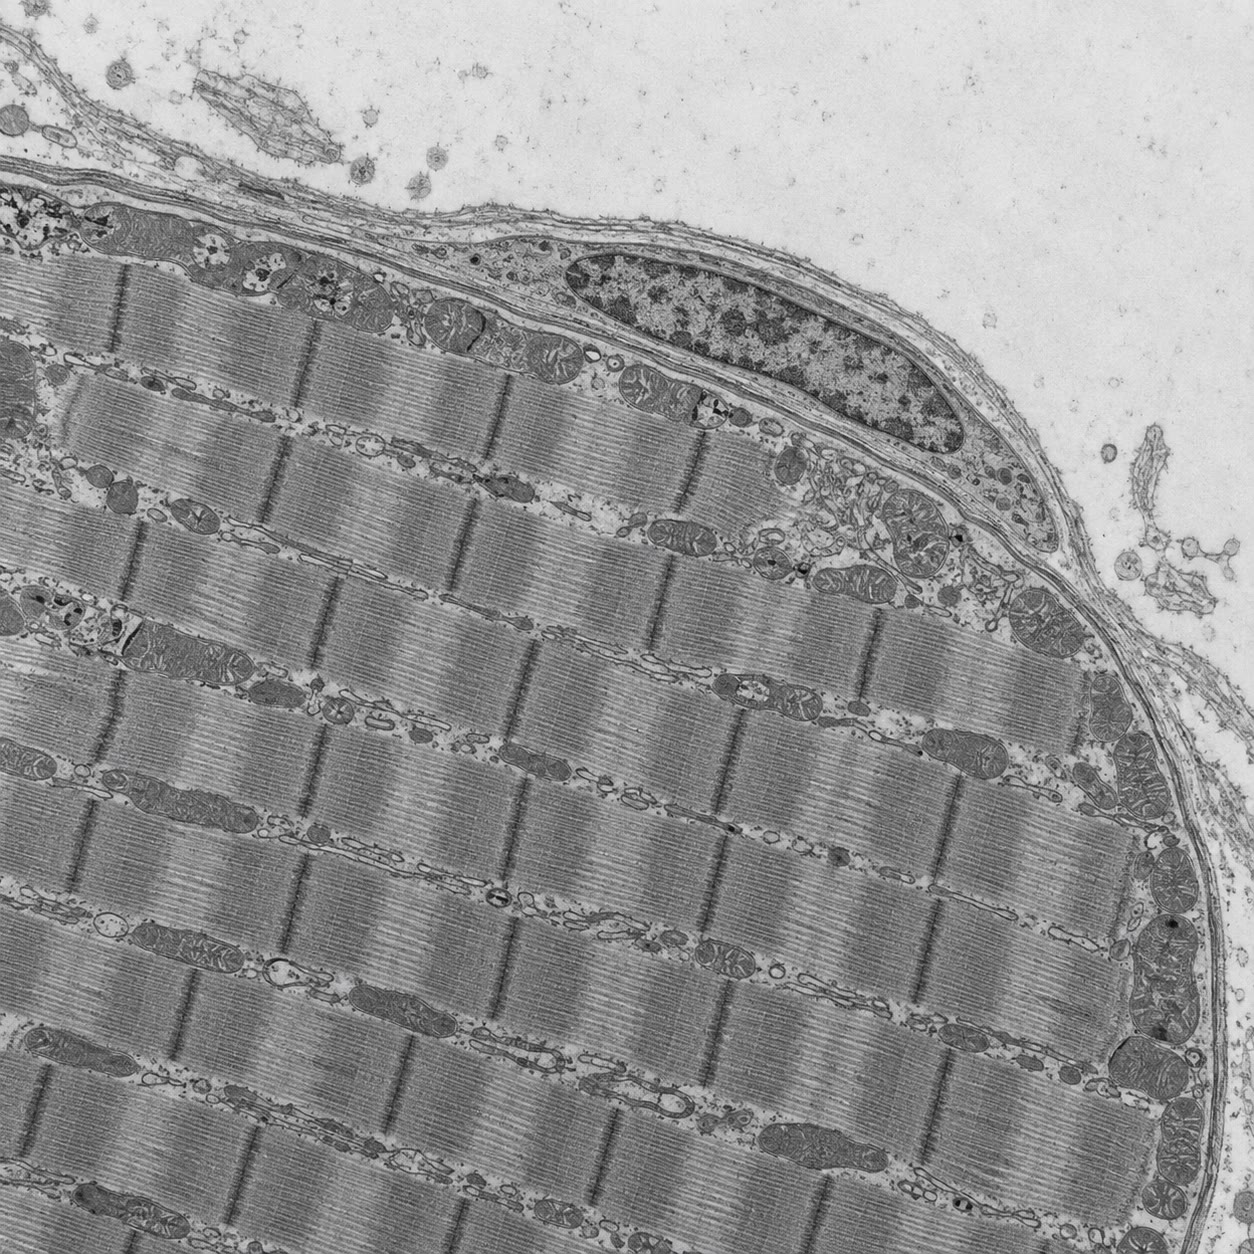
\includegraphics[width=0.42\linewidth]{images/book4/ai/b4-12-satellite-cell-tem.jpg}

{\small Una célula satélite al microscopio electrónico: una pequeña célula
mononucleada alojada entre la membrana de una \omterm{def:b2:cell-differentiation:myogenesis}{fibra muscular} y su lámina
basal --- la reserva de \omterm{def:b2:cell-differentiation:myogenesis}{mioblastos} de la fibra.}
\end{omfigure}

\section{Ejercicios}

\begin{exercise}[$\star$]\label{exo:b2:cell-differentiation:1}
Defínanse \omterm{def:b2:cell-differentiation:differentiation}{diferenciación}, \omterm{def:b2:cell-differentiation:differentiation}{determinación} y \omterm{def:b2:cell-differentiation:differentiation}{potencia}, y sitúense el cigoto,
una célula de la \omterm{def:b2:mammal-reproduction:implantation}{masa celular interna}, una célula satélite y una \omterm{def:b2:cell-differentiation:myogenesis}{fibra
muscular} en la escala de \omterm{def:b2:cell-differentiation:differentiation}{potencia}.
\end{exercise}

\begin{exercise}[$\star$]\label{exo:b2:cell-differentiation:2}
Enumérense las etapas de la miogénesis, de la célula del somito a la \omterm{def:b2:cell-differentiation:myogenesis}{fibra
muscular}, con el \omterm{prop:b2:cell-differentiation:transcriptional}{factor de transcripción} que se expresa en cada una.
\end{exercise}

\begin{exercise}[$\star$]\label{exo:b2:cell-differentiation:3}
¿Qué mostró el trasplante nuclear de Gurdon, y qué no mostró?
\end{exercise}

\begin{exercise}[$\star$]\label{exo:b2:cell-differentiation:4}
Nómbrense las partes de un \omterm{def:b2:cell-differentiation:fibre}{sarcómero} y dígase cuáles se mueven y cuáles no
cuando la fibra se acorta.
\end{exercise}

\begin{exercise}[$\star\star$]\label{exo:b2:cell-differentiation:5}
Una fibra de \qty{20}{cm} de largo tiene \omterm{def:b2:cell-differentiation:fibre}{sarcómeros} de \qty{2.5}{\micro m}
y un núcleo cada \qty{25}{\micro m} de longitud. ¿Cuántos \omterm{def:b2:cell-differentiation:fibre}{sarcómeros} hay
en serie, y cuántos núcleos? ¿Cuántos \omterm{def:b2:cell-differentiation:myogenesis}{mioblastos} se fusionaron para
formarla?
\end{exercise}

\begin{exercise}[$\star\star$]\label{exo:b2:cell-differentiation:6}
Explíquese por qué los \omterm{def:b2:cell-differentiation:myogenesis}{mioblastos} no se fusionan mientras hay FGF, a
partir del inhibidor Id, y predígase qué les ocurre a unos \omterm{def:b2:cell-differentiation:myogenesis}{mioblastos}
modificados para fabricar Id de forma constitutiva.
\end{exercise}

\begin{exercise}[$\star\star$]\label{exo:b2:cell-differentiation:7}
En el modelo del interruptor con $a = 1$, $K = 1$, $b = 0.02$ y $k = 0.4$,
compruébese por sustitución que $m = 2.1$ está cerca de un estado
estacionario, hállese aproximadamente el estado estacionario bajo y
dígase qué le ocurre a una célula cuya $m$ se eleva brevemente a $1$ y
después se deja evolucionar libremente.
\end{exercise}

\begin{exercise}[$\star\star$]\label{exo:b2:cell-differentiation:8}
En el mismo modelo, $k$ se eleva a $0.6$ (el factor se degrada más
deprisa). Muéstrese gráfica o numéricamente que el estado alto
desaparece. ¿Qué predice esto para una célula en la que \omterm{def:b2:cell-differentiation:myogenesis}{MyoD} está
desestabilizado?
\end{exercise}

\begin{exercise}[$\star\star$]\label{exo:b2:cell-differentiation:9}
Predígase el \omterm{def:b2:meiosis-heredity:vocabulary}{fenotipo} de un ratón que carece de (a) \omterm{def:b2:cell-differentiation:myogenesis}{MyoD} y Myf5 a la vez,
(b) solo miogenina, (c) solo \omterm{def:b2:cell-differentiation:myogenesis}{MyoD}. ¿Por qué (c) es casi normal?
\end{exercise}

\begin{exercise}[$\star\star\star$]\label{exo:b2:cell-differentiation:10}
Un fibroblasto transfectado con \omterm{def:b2:cell-differentiation:myogenesis}{MyoD} se convierte en un \omterm{def:b2:cell-differentiation:myogenesis}{miotubo}; una
célula hepática transfectada con \omterm{def:b2:cell-differentiation:myogenesis}{MyoD} no. Propóngase una explicación que
implique la cromatina y la competencia, y un experimento para
comprobarla.
\end{exercise}

\begin{exercise}[$\star\star\star$]\label{exo:b2:cell-differentiation:11}
El entrenamiento de resistencia convierte fibras rápidas hacia fibras
lentas sin cambiar su genoma. Explíquese, en términos de expresión génica,
cómo puede hacerlo el patrón de descargas del nervio, y por qué las fibras
siguen siendo, pese a todo, músculo esquelético y nunca se convierten,
por ejemplo, en cartílago.
\end{exercise}

\begin{exercise}[$\star\star\star$]\label{exo:b2:cell-differentiation:12}
``Una célula diferenciada recuerda lo que es con un circuito, no con una
\omterm{def:b2:genome-diversification:mutation}{mutación}.'' Discútase a partir del interruptor biestable, de la cromatina
y del hecho de que los reinicios de Gurdon y de Yamanaka son posibles pero
poco eficaces.
\end{exercise}

\section{Problema: un músculo construido y reconstruido}

\begin{problem}[{Problema de fin de semana --- un músculo seguido desde el
somito hasta la fibra y a través de una lesión: el número de mioblastos,
de fusiones y de núcleos, el análisis del interruptor biestable, el
calendario de una reparación y la cuantificación del entrenamiento, hasta
llegar al número de núcleos de la fibra, el umbral del interruptor y el
tiempo de reparación}]
\label{pb:b2:cell-differentiation:1}
Un músculo del muslo de un adulto tiene \num{500000} fibras, cada una de
\qty{20}{cm} de largo y \qty{60}{\micro m} de diámetro, con un núcleo por
cada \qty{25}{\micro m} de longitud; los \omterm{def:b2:cell-differentiation:fibre}{sarcómeros} miden
\qty{2.5}{\micro m}. Los \omterm{def:b2:cell-differentiation:myogenesis}{mioblastos} embrionarios se dividen cada
\qty{12}{h} mientras hay FGF. Modelo del interruptor: $a = 1$, $K = 1$,
$b = 0.02$, $k
= 0.4$. Tras una lesión que destruye el \qty{10}{\%} de la longitud de
cada fibra, las células satélite del segmento lesionado (\num{4} por
milímetro de fibra) se dividen cada \qty{18}{h} durante un tiempo y
después se fusionan.

\medskip
\noindent\textbf{Parte I --- La fibra.}
\begin{enumerate}
  \item Calcúlense el número de \omterm{def:b2:cell-differentiation:fibre}{sarcómeros} en serie de una fibra y el
        número de núcleos.
  \item ¿Cuántos \omterm{def:b2:cell-differentiation:myogenesis}{mioblastos} se fusionaron para formar una fibra? ¿Y todo
        el músculo?
  \item Calcúlense el volumen de una fibra y el del músculo (en litros).
  \item Estímese el volumen citoplasmático que atiende cada núcleo, y
        compárese con una célula ordinaria de \qty{2000}{\micro m^3}.
  \item ¿Por qué se sitúan los núcleos en la periferia de una fibra
        madura?
  \item Los \omterm{def:b2:cell-differentiation:myogenesis}{mioblastos} del músculo descienden de \num{2000} células del
        somito. ¿Cuántas duplicaciones necesitaron, y cuántos días, para
        alcanzar el número de la pregunta 2?
\end{enumerate}

\medskip
\noindent\textbf{Parte II --- El interruptor.}
\begin{enumerate}[resume]
  \item Escríbase la condición de estado estacionario y muéstrese que $m \approx
        0.055$ la cumple.
  \item Muéstrese que $m \approx 2.1$ la cumple.
  \item Muéstrese que hay una tercera solución cerca de $m = 0.41$, y
        explíquese a partir de los signos de $\mathrm{d}m/\mathrm{d}t$ a
        ambos lados que es inestable.
  \item Un pulso de inductor eleva $m$ a $0.6$; otro, a $0.3$. ¿Cuál es el
        destino de cada célula?
  \item Una \omterm{def:b2:genome-diversification:mutation}{mutación} eleva la síntesis basal $b$ a $0.4$. Muéstrese que el
        estado bajo desaparece. ¿Qué hace la célula?
  \item Explíquese cómo explica este modelo que el compromiso sobreviva a
        la división celular, y qué debe ser cierto de $m$ en cada división.
\end{enumerate}

\medskip
\noindent\textbf{Parte III --- La reparación.}
\begin{enumerate}[resume]
  \item ¿Cuántas células satélite lleva una fibra, y cuántos núcleos hay
        que sustituir tras la lesión?
  \item ¿Cuántas duplicaciones deben realizar las células satélite para
        aportarlos, y cuánto tiempo lleva eso?
  \item Compárese con las dos o tres semanas observadas para la
        reparación, y dígase qué más incluye ese tiempo.
  \item ¿Por qué deben las células satélite volver a expresar \omterm{def:b2:cell-differentiation:myogenesis}{MyoD} antes de
        fusionarse, y por qué deben dejar antes de dividirse?
  \item Cada ronda de reparación consume algunas células satélite. Si la
        reserva disminuye un \qty{5}{\%} por lesión, ¿cuántas lesiones
        hacen falta para reducirla a la mitad?
  \item ¿Cuántas células satélite por fibra quedan tras veinte lesiones
        de este tipo?
  \item Explíquese por qué un músculo distrófico, cuyas fibras se
        desgarran en cada contracción, es sustituido por tejido fibroso al
        cabo de años.
\end{enumerate}

\medskip
\noindent\textbf{Parte IV --- El entrenamiento.}
\begin{enumerate}[resume]
  \item El entrenamiento engrosa cada fibra hasta \qty{80}{\micro m}. ¿En
        qué factor crece el volumen de la fibra, y cuántos núcleos
        adicionales deben aportar las células satélite si se mantiene la
        proporción de la pregunta 4?
  \item Calcúlese el nuevo volumen del músculo.
  \item El entrenamiento de resistencia convierte el \qty{30}{\%} de las
        fibras rápidas en lentas. ¿Qué ha cambiado en esas fibras y qué no?
  \item Explíquese por qué un músculo adulto aumenta de tamaño por
        crecimiento de las fibras y no por adición de fibras, a partir del
        hecho de que las fibras no se dividen.
  \item Un fármaco bloquea la fusión de las células satélite. Predígase la
        respuesta del músculo al entrenamiento y a una lesión.
  \item Enúnciese el resultado: el número de núcleos de la fibra, el umbral
        del interruptor y el tiempo que tardan las células satélite en
        aportar los núcleos de una reparación.
\end{enumerate}
\end{problem}
